%\documentclass[prl,superscriptaddress,showpacs,floatfix,twocolumn]{revtex4}
\documentclass[aps,showpacs,floatfix,nofootinbib,preprintnumbers,superscriptaddress,amsmath,amssymb]{revtex4-1}
%\documentclass[prl,superscriptaddress,showpacs,floatfix]{revtex4}
\usepackage{graphicx,amsmath,amssymb,bm}
\usepackage{amsfonts}
\usepackage{color}
\usepackage{float}
\usepackage{dcolumn}
\usepackage{subfigure}
\usepackage{multirow} 

\newcommand{\bra}[1]{\left\langle #1 \right|}
\newcommand{\ket}[1]{\left| #1 \right\rangle}

\begin{document}

\title{Evolution of single-particle energies, two and many-body forces and all that}
\author{A.~Ekstr\"om}
\affiliation{Department of Fundamental Physics, Chalmers University of Technology, SE-412 96 G{\"o}teborg, Sweden}
\author{G.~R.~Jansen}
\affiliation{Department of Physics and Astronomy, University of
Tennessee, Knoxville, TN 37996, USA}
\affiliation{Physics Division, Oak Ridge National Laboratory,
Oak Ridge, TN 37831, USA}
\author{G.~Hagen}
\affiliation{Physics Division, Oak Ridge National Laboratory,
Oak Ridge, TN 37831, USA}
\affiliation{Department of Physics and Astronomy, University of
Tennessee, Knoxville, TN 37996, USA}
\author{M.~Hjorth-Jensen}
\affiliation{Department of Physics, University of Oslo, N-0316 Oslo, Norway}
\affiliation{National Superconducting Cyclotron Laboratory and Department of Physics and Astronomy, Michigan
  State University, East Lansing, MI 48824-1321, USA}
\author{T.~Papenbrock} 
\affiliation{Department
  of Physics and Astronomy, University of Tennessee, Knoxville, TN
  37996, USA} 
\affiliation{Physics Division, Oak Ridge National
  Laboratory, Oak Ridge, TN 37831, USA} 

\begin{abstract}
\begin{description}
 \item[Background] To get a proper handle on correlations in nuclear systems and relate
these to the underlying forces, forms an essential part in basic
nuclear physics research and has wide ranging implications for our
understanding of how subatomic matter organizes itself and what
phenomena emerge. To identify the mechanisms which are
responsible for the occurence or not of so-called magic numbers in
various regions of the nuclear chart, requires systematic studies of
correlations and nuclear forces.
 \item[Purpose] In this work we analyze the evolution of effective
   single-particle energies for the chain of oxygen, calcium, nickel
   and tin isotopes and study the role of two- and three-body forces
   in terms of their central, spin-orbit and tensor force components.
   The aim is to understand the role of these components towards the
   respective driplines of the above isotopic chains. Nuclear forces
   based on chiral effective field theory and systematically fit to
   nuclear data are employed in these studies.
 \item[Methods] We have carried out studies of the single-particle
   energies using a spin-tensor decomposition of the nuclear
   forces. The effective single-particle energies have been computed using
   Hartree-Fock theory, many-body perturbation theory and
   coupled-cluster theory with recently fitted nuclear forces.  The
   nuclear forces have been fitted to the available body of
   experimental data using the model-based, derivative-free
   optimization algorithm POUNDerS developed at Argonne National
   Laboratory.  We optimize the chiral interaction at next-to-next-to
   leading order (NNLO).
 \item[Results] 
 \item[Conclusions]
\end{description}
\end{abstract}

\pacs{21.10.-k, 21.10.Dr, 21.30.Fe, 21.60.De}

\maketitle 


\section{Introduction}\label{sec:intro}

The understanding of nuclear structure and reactions and thereby
properties of nuclei in terms of the underlying strong force and the
pertinent laws of motion, involves a number of approximations that
pose a great challenge to nuclear theory.  Similarly, our interpretations of
experimentally measurable quantities rely as well on several assumptions and
approximations.  As an example, concepts such as an independent
particle motion and various mean-field approaches based thereupon,
play an important role in the analysis and interpretation of
experimental results. Eventual deviations from such a mean-field
picture are interpreted as a possible measure of correlations, with
the potential of providing a better understanding of the role of the
underlying strong force in a nuclear many-body environment.  A popular
theoretical approach for studying correlations beyond a given mean field, is
the nuclear shell model, see for example
Refs.~\cite{lawson1980,talmi1993,caurier2005}. It rests on the assumption that the
state functions used in nuclear structure studies can be approximated
by various Slater determinants based on a particular orthonormal set of
single-particle states. The shell model has been rather successful in
describing many of the observed features of nuclei and experimental
probes like nucleon transfer and knockout reactions have been
essential in supporting a mean-field picture of
nuclei. Single-particle properties have been extracted by measurements
of nucleon-adding and nucleon-removing transfer reactions,
establishing thereby a link between observables and theoretical
interpretations, see for example
Refs.~\cite{schiffer2012,schiffer2013} and discussions therein. 


However, in nuclear physics, the analysis and theoretical
interpretations of correlations beyond a mean field picture are
complicated by the fact that the strong force is represented by
various effective models and Hamiltonians in the energy regime of
nuclear structure studies. These effective Hamiltonians are nowadays
based on  chiral effective field theory
(EFT),  see for example
Refs.~\cite{weinberg1990,weinberg1991,ordonez1992,ordonez1994,ordonez1996,vankolck1999,machleidt2011,epelbaum2009,ekstrom2013}.  
The EFT nuclear interactions that are currently
employed in nuclear structure calculations employ normally pions and nucleons
as effective degrees of freedom. Compared
with former interaction models inspired by a one-boson-exchange
approximation (see Refs.~\cite{machleidt1989,machleidt2001} for
relevant reviews), interactions based on chiral EFT exhibit currents
that are consistent with the underlying Lagrangian that defines the
interactions. Furthermore, chiral EFT interactions allow for systematic
improvements since they are based on power counting in terms of the
probed momentum scale over a given cutoff scale $\Lambda$.  The power counting
introduces also a systematic recipe for constructing nucleon-nucleon
($NN$) forces, three-nucleon ($3N$) forces, and forces of higher rank.

To get a proper handle on correlations in nuclear systems and relate
these to the abovementioned underlying forces, forms an essential part
in basic nuclear physics research and has wide ranging implications
for our understanding of how subatomic matter organizes itself and
what phenomena emerge. For example, to identify the mechanisms which
are responsible for the occurence or not of so-called magic numbers in
various regions of the nuclear chart, will most likely require
systematic studies of correlations beyond standard shell-model
calculations, which often are limited to one or at most two major
oscillator shells.  For exotic isotopes close to the so-called drip
lines, continuum degrees of freedom and more complicated many-body
forces may become important, as demonstrated recently in
Refs.~\cite{hagen2012a,hagen2012b} for the chains of oxygen and
calcium isotopes.  

The $NN$ interaction has traditionally been studied
in terms of its central, spin-orbit and tensor force.  These terms
accomodate to a large degree our phenomenological knowledge of the
strong interaction, which, when applied in a nuclear many-body
context, is subjected to various degrees of renormalization.  In
particular, the tensor force, a non-central component of the nuclear
force, has been shown to play an important role for the development of
magic numbers of nuclei with large $N/Z$ ratios, see
Refs.~\cite{otsuka2001,otsuka2005,otsuka2010b,tsunoda2011,smirnova2010}.
Furthermore, the spin-orbit force which arises from the nuclear
forces, is of the order of the average binding energy per
nucleon and plays an important role in defining nuclear
single-particle fields. Its importance is essential in order to account
for magic numbers and large shell gaps in nuclei and lead, in the
early days of nuclear physics, to the introduction of an empirical
one-body spin-orbit force \cite{mayer1949,haxel1949}. To relate such
an empirical spin-orbit force to the underlying nuclear forces is an
unresolved and outstanding problem in nuclear physics, see for example
Refs.~\cite{ando1981,burgunder2014}.  In
Refs.~\cite{ando1981,pieper1993}, the large splittings in energy
between states that can be interpreted as representing single-particle
spin-orbit partners in for $A=15$ and $A=39$, could be related both to
the two-body spin-orbit force and a contribution to the spin-orbit
force from three-body forces. In Ref.~\cite{pieper1993}, the authors
showed that the two-nucleon spin-orbit force gave approximately half
of the observed splitting, while the other half came from pion
exchange interactions between three or more nucleons.

In order to shed light on these issues, we present in this work an
analysis of effective single-particle energies and their evolution as
function of neutron numbers for selected oxygen, calcium, nickel and
tin isotopes. The interactions which define the single-particle
energies contain two-body and three-body forces defined within the
framework of chiral effective field theory.  We optimize the chiral
interaction up to next-to-next-to leading order (NNLO) using the
recently developed model-based, derivative-free algorithm POUNDerS
\cite{taoman}.  The cutoff dependence of the chiral forces and the
various optimizations allow us in turn to study the convergence
properties of chiral forces in a nuclear many-body
environment. Furthrmore, these interactions are in turn decomposed in
terms of a central, spin-orbit and tensor force
component~\cite{elliott1968,kirson1973,brown1988,osnes1992,richter1991,smirnova2010}. This
decomposition allows thereby for a systematic analysis of the
spin-orbit force and the tensor force as functions of varying neutron
and proton numbers.  The single-particle energies for the above
isotopes are computed using Hartree-Fock theory, many-body
perturbation theory and coupled-cluster theory
\cite{shavittbartlett2009}. The effective single-particle energies are defined
as one particle (protons and neutrons) on top of nuclei with
$j$-filled shells. Although this definition of an effective single-particle
energy is questionable, see for example the discussion in
Ref.~\cite{duguet2012}, it has been widely used in a 
nuclear structure, see for example
Refs.~\cite{otsuka2005,otsuka2010b,smirnova2010,nowacki2012,smirnova2012,sorlin2008}.

After these introductory remarks, we present in the next section our
theoretical framework, with the definition of effective
single-particle energies and their relation to the decomposition of
the nuclear forces in central, spin-orbit and tensor components. The
nuclear interactions we include in our analysis are only briefly
reviewed here. Where details are needed, we refer the reader to our
recent parametrization of chiral forces in
Ref.~\cite{carlsson2014}. Section \ref{sec:results} presents our main
findings while Sec.~\ref{sec:conclusions} outlines our conclusions
and perspectives.






 
\section{Theoretical framework}\label{sec:formalism}

In this section we present first our basic definitions of Hamiltonians
with and without three-body forces and link these expressions with the
derivation the so-called monopole interaction and its connection with
single-particle energies at a mean-field level. The interactions are
in turn analyzed in terms of a multi-component expansion of the
nuclear forces, with an emphasis of the central, spin-orbit and tensor
components. These terms accomodate our basic phenomenological
knowledge of the strong interaction. We end this section with a
summary on how to parametrize chiral interactions. These interactions,
which are constrained to reproduce several nuclear observables via an
optimization procedure, form the input to our analysis.
 
\subsection{Definitions}\label{subsec:definitions}

Our Hamiltonian contains one-body, two-body and three-body contributions and in 
the equations below, we  label states below the Fermi level $F$ as $i,j,\ldots$ while states 
above the Fermi level are defined by $a,b,\ldots$. General single-particle states
are given by the letters  $p,q \dots$. The
quantities $pq\dots$ represent the quantum numbers of various
single-particle states, namely
$p=(n_p,l_p,j_p,m_{j_p},t_{z_p})$.   
The commutation relations for creation and annihilations operators with respect to
a given reference state are then given by
\[
   \left\{a_p^\dagger, a_q \right\}= \delta_{pq}, p, q \leq F \hspace{0.5cm} \left\{a_p, a_q^\dagger \right\} =
        \delta_{pq}, p, q > F.
\]
The action of the creation and annihilation operators with respect to a reference state $\Phi_0$ are then given by
 $a_i|\Phi_0\rangle = |\Phi_i\rangle$ where a state labeled by $|\Phi_i\rangle$ means that a particle in a 
single-particle state $i$ has been removed. Similarly, we have $a_a^\dagger|\Phi_0\rangle = |\Phi^a\rangle$, $a_i^\dagger|\Phi_0\rangle = 0$ 
and $a_a|\Phi_0\rangle = 0$.  With the above definitions, we write our Hamiltonian as
\[
\hat{H}=\hat{H}_0+\hat{V}+\hat{W},
\]
where 
the single-particle part is given by
 \[
    \hat{H}_0 = \sum_{pq} \langle p|\hat{h}_0|q\rangle a_p^\dagger a_q.
 \]
This part of the Hamiltonian is commonly defined in terms of some external potential like the three-dimensional 
harmonic oscillator or a particular mean-field basis. 
Similarly, the two-body part of the Hamiltonian
is given by  
\[
  \hat{V} = \frac{1}{4}\sum_{pqrs} \langle pq|\hat{v}|rs\rangle_{\mathrm{AS}} a_p^\dagger a_q^\dagger a_s a_r
\]
where we have employed antisymmetric matrix elements defined as
\[
\langle pq|\hat{v}|rs\rangle_{\mathrm{AS}}=\langle pq|\hat{v}|rs\rangle-\langle pq|\hat{v}|sr\rangle.
\]
We will assume throughout this work that the  two-body operator $\hat{v}$ is given by a nucleon-nucleon interaction.
The models for the two-nucleon interaction will be defined in Sec.~\ref{subsec:forcemodels}. 
Finally, the three-body part of our Hamiltonian operator  is defined by   
\[
   \hat{W} =\frac{1}{36} \sum_{pqrstu} \langle pqr|\hat{w}|stu\rangle_{\mathrm{AS}}a_p^\dagger a_q^\dagger a_r^\dagger a_u a_t a_s,
\]
where we have defined the antisymmetric matrix elements
\[
          \langle pqr|\hat{w}|stu\rangle_{\mathrm{AS}}= \langle pqr|\hat{w}|stu\rangle + \langle pqr|\hat{w}|tus\rangle + \langle pqr|\hat{w}|ust\rangle- \langle pqr|\hat{w}|sut\rangle - \langle pqr|\hat{w}|tsu\rangle - \langle pqr|\hat{w}|uts\rangle.
\]
We will in the discussions to come drop the $\mathrm{AS}$ subscript,
assuming thereby that all matrix elements are antisymmetrized.
Introducing a reference state $|\Phi_0\rangle$ as our new vacuum state
leads to a redefinition of the Hamiltonian in terms of a constant
reference energy $E_0$ defined as
\[
E_0 = \sum_{i\le F}\langle i | \hat{h}_0|i\rangle+\frac{1}{2}\sum_{ij\le F} \langle ij|\hat{v}|ij\rangle +\frac{1}{6}\sum_{ijk\le F} \langle ijk|\hat{w}|ijk\rangle,
\]
and a normal-ordered Hamiltonian 
\[
  \hat{H}_N=\sum_{pq}\langle p|\tilde{f}|q\rangle a^\dagger_p a_q+\frac{1}{4} \sum_{pqrs} \langle pq|\tilde{v}|rs\rangle a^\dagger_p a^\dagger_q a_s  a_r +\frac{1}{36} \sum_{\substack{pqr \\stu}}
                 \langle pqr|\hat{w}|stu\rangle a^\dagger_p a^\dagger_q a^\dagger_r a_u a_t a_s 
\]
where
\[
\langle p| \tilde{f}|q\rangle = \langle p|\hat{h}_0|q\rangle +\sum_{i\le F} \langle pi|\hat{v}|qi\rangle+\frac{1}{2}\sum_{ij\le\alpha_F} \langle pij|\hat{w}|qij\rangle,
\] 
represents a correction to the single-particle operator $\hat{h}_0$ due to contributions from the nucleons below the Fermi level.
The two-body matrix elements are now modified in order to account for medium-modified contributions from the three-body interaction, resulting in
\begin{equation}
\langle pq|\tilde{v}|rs\rangle=\langle pq|\hat{v}|rs\rangle+\sum_{i\le F} \langle pqi|\hat{w}|rsi\rangle.
\label{eq:twobodyveff}
\end{equation}
In Eq.~(\ref{eq:twobodyveff}), the effective two-body interaction
$\tilde{v}$ can contain both a standard two-nucleon interaction and a
density dependent contribution stemming from a three-body interaction
$\hat{w}$.

An important ingredient in studies of effective interactions and their
applications to nuclear structure, is the so-called monopole
interaction, normally defined in terms of a nucleon-nucleon
interaction $\hat{v}$ \cite{otsuka2001,otsuka2005,otsuka2010b,smirnova2010,nowacki2012,smirnova2012,sorlin2008,poves1981a,poves1981b,zuker2003}
\begin{equation}
\bar{V}_{\alpha_p\alpha_q} = \frac{\sum_{J}(2J+1) \langle (\alpha_p\alpha_q)J | \hat{v} | (\alpha_p\alpha_q)J \rangle }{\sum_{J}(2J+1)},
\label{eq:monopole1}
\end{equation}
where the total angular momentum of a two-body state $J$ runs over all
possible values.  
In the above equation we have defined a nucleon-nucleon interaction in a so-called angular-momentum 
coupled representation with the symbol $\alpha_{p,q}$ representing all possible quantum numbers except the 
magnetic substates $m_{j_{p,q}}$
The monopole Hamiltonian can be interpreted as an angle-averaged matrix element.  
We have assumed that the single-particle angular momenta $j_p$ and $j_q$ couple to a total
two-particle angular momentum $J$.  The summation over $J$ with the value $2J+1$ can be replaced
by $\sum_J(2J+1)=(2j_p+1)(2j_q+1)$ if $\alpha_p\ne \alpha_q$. If $\alpha_p=\alpha_q$ we can generalize this equation to, assuming that 
our states can represent either protons or neutrons,
\begin{equation}
\sum_{J}(2J+1)=(2j_p+1)(2j_q+1-\delta_{\alpha_p\alpha_q}).
\label{eq:jvalue}
\end{equation}
The spherical single-particle states,
provide an important ingredient for the formation of shells and
interplay between spherical configurations and deformation in
nuclei. Large shell gaps obtained from a monopole Hamiltonian are a
prerequisite to obtain certain magic numbers. 
Equation~(\ref{eq:monopole1}) can also be expressed in terms of the
medium-modified two-body interaction defined in
Eq.~(\ref{eq:twobodyveff}), that is we can have 
\begin{equation}
\tilde{V}_{\alpha_p\alpha_q} = \frac{\sum_{J}(2J+1) \langle (\alpha_p\alpha_q)J | \tilde{v} | (\alpha_p\alpha_q)J \rangle }{\sum_{J}(2J+1)}.
\label{eq:monopole2}
\end{equation}
As stated in the introduction, one of the
aims of this work is to study the role of three-body interactions in
nuclear structure, with an emphasis on the evolution of
single-particle energies.


The single-particle energy $\epsilon_p$ resulting from for example a self-consistent Hartree-Fock field, 
or from  first order in many-body perturbation theory, is given by (in an uncoupled basis)
\[
\epsilon_p=\langle p| \tilde{f}|p\rangle = \langle p|\hat{h}_0|p\rangle +\sum_{i\le F} \langle pi|\hat{v}|pi\rangle+\frac{1}{2}\sum_{ij\le\alpha_F} \langle pij|\hat{w}|pij\rangle,
\]
where we have included the three-body interaction as well.
We can rewrite this equation in an angular coupled basis ($jj$-coupled basis) as 
\begin{equation}
\epsilon_{\alpha_p}= \langle \alpha_p|\hat{h}_0|\alpha_p\rangle+\frac{1}{2j_p+1}\sum_{\alpha_i\le \alpha_F}\sum_{J} (2J+1)\langle (\alpha_p\alpha_i)J | \hat{v} | (\alpha_p\alpha_i)J \rangle,
\label{eq:spequation1}
\end{equation}
or
\begin{equation}
\epsilon_{\alpha_p}= \langle \alpha_p|\hat{h}_0|\alpha_p\rangle+\frac{1}{2j_p+1}\sum_{\alpha_i\le \alpha_F}\sum_{J} (2J+1)\langle (\alpha_p\alpha_i)J | \tilde{v} | (\alpha_p\alpha_i)J \rangle,
\label{eq:spequation2}
\end{equation}
where the first equation contains a two-body force only while
Eq.~(\ref{eq:spequation2}) includes the medium-modified contribution
from the three-body interaction as well. In
Eqs.~(\ref{eq:spequation1}) and (\ref{eq:spequation2}), we have
used a compact notation for the single-particle states, with the
symbol $\alpha_p$ etc representing all possible quantum numbers except
the magnetic substates $m_{j_p}$, that is $\alpha_p=(n_p,l_p,j_p,t_{z_p})$. The symbol $\alpha_F$ stands now for
all single-particle states up to the Fermi level, excluding again the
magnetic substates.  In the above two-body interaction matrix elements
$\langle (\alpha_p\alpha_i)J | \hat{v}(\tilde{v}) |(\alpha_p\alpha_i)J \rangle$ we have dropped additional quantum
numbers like the isospin projection. Our interactions are diagonal in
the projection of the total isospin but breaks both isospin symmetry
and charge symmetry.

Depending on the choice of single-particle Hamiltonian, the quantity
$\langle \alpha_p|\hat{h}_0|\alpha_p\rangle$ could represent the expectation value of the single-particle
kinetic energy or the eigenstate of a single-particle Hamiltonian
$\hat{h}_0$. The latter could for example be the solution of
Schr\"odinger's equation for a particle moving in a Woods-Saxon like
single-particle potential, or the widely employed harmonic oscillator
in three dimensions.

Using the definition of the single-particle energy in
Eq.~(\ref{eq:spequation1}), the definition of the monopole matrix
element in Eqs.~(\ref{eq:monopole1}) or (\ref{eq:monopole2}) and Eq.~(\ref{eq:jvalue}), we can rewrite
Eq.~(\ref{eq:spequation1}) as
\begin{equation}
\epsilon_{\alpha_{p}}=\langle \alpha_p|\hat{h}_0|\alpha_p\rangle+\sum_{\alpha_i\le \alpha_F}N_{\alpha_i}\bar{V}_{\alpha_p\alpha_i},
\label{eq:spmono1}
\end{equation}
with $N_{\alpha_i}=2\alpha_i+1$, and Eq.~(\ref{eq:spequation2}) as 
\begin{equation}
\epsilon_{\alpha_{p}}=\langle \alpha_p|\hat{h}_0|\alpha_p\rangle+\sum_{\alpha_i\le \alpha_F}N_{\alpha_i}\tilde{V}_{\alpha_p\alpha_i}.
\label{eq:spmono2}
\end{equation}




\subsection{Spin-tensor decomposition}\label{subsec:spintensor}

The effective interaction discussed in the previous subsection is a
scalar two-body operator. A general scalar two-body operator
$\hat{v}$ can be written as
\begin{equation}
\hat{v} = \sum_{k} \hat{v}_{k} = \sum_{k} \mbox{\boldmath $C^{(k)}\cdot
Q^{(k)}$},
\end{equation}
where the operators \mbox{\boldmath $C^{(k)}$} and
\mbox{\boldmath $Q^{(k)}$} are irreducible spherical tensor
operators of rank $k$, acting in spin and coordinate space,
respectively. The value of $k$ is limited to $k\le 2$ since the total eigenspin of the two-nucleon
system is either $0$ or $1$. The term with
$k=0$ refers to the central component of the two-body
operator.
The values of $k=1$ and $k=2$ are called
the vector and the tensor components, respectively. The vector term is also called the two-body spin-orbit term, although it
also contains the anti-symmetric spin-orbit term, see for example Ref.~\cite{conze1973} for further details.
Using standard angular momentum algebra it is rather straightforward to relate the matrix elements  $\hat{v}_{k}$ to
those of say $\hat{v}$ or $\tilde{v}$. 

One possible decomposition of the effective interaction is to
express the $k$-th component of the interaction $\langle
(\alpha_p\alpha_q)J|\hat{v}_{k}|(\alpha_r\alpha_s)J\rangle $ in a $jj$-coupled basis, where
$\hat{v}_k$ is related to the matrix
elements $\langle (\alpha_p\alpha_q)J|\hat{v}|(\alpha_r\alpha_s)J\rangle $ (or $\langle (\alpha_p\alpha_q)J|\tilde{v}|(\alpha_r\alpha_s)J\rangle $ 
through the relation
\begin{eqnarray}
\langle (\alpha_p\alpha_q)J|\hat{v}_{k}|(\alpha_r\alpha_s)J\rangle&=&(-1)^{J}(2k+1)
\sum_{LL'SS'}\langle
\alpha_p\alpha_q|LSJ\rangle \langle \alpha_r\alpha_s|L'S'J\rangle
\left\{ \begin{array}{ccc}
		       L&S&J\\
		       S'&L'&k
		       \end{array}
		 \right\} \nonumber \\
& &\times \sum_{J'}(-1)^{J'}(2J'+1)\left\{ \begin{array}{ccc}
		       L&S&J'\\
		       S'&L'&k
		       \end{array}
		 \right\}
\sum_{\alpha_{p}'\alpha_{q}'\alpha_{r}'\alpha_{s}'}\langle \alpha_p'\alpha_q'|LSJ'\rangle
\nonumber\\
& &\times \langle \alpha_r'\alpha_s'|L'S'J'\rangle \langle
(\alpha_p'\alpha_q')J'|\hat{v}|(\alpha_r'\alpha_s')J'\rangle .  \label{eq:jj}
\end{eqnarray}
The two-particle matrix elements are normalized and antisymmetrized.
A similar expression applies to the medium-modified two-body interaction $\tilde{v}$ of 
Eq.~(\ref{eq:twobodyveff}) as well.
The symbol $\langle \alpha_p\alpha_q|LSJ \rangle $ is a shorthand
for the $LS-jj$ transformation coefficient,
\[
\langle \alpha_p\alpha_q|\lambda SJ \rangle = \sqrt{(2j_{p}+1)(2j_{q}+1)(2\lambda+1)(2S+1)}
\left\{
\begin{array}{ccc}
       l_{p}&\frac{1}{2}&j_{p}\\
       l_{q}&\frac{1}{2}&j_{q}\\
       \lambda    &S          &J
\end{array}
\right\},
\]
see for example Ref.~\cite{lawson1980}. 
The transformation from an $LS$ basis to a $jj$-coupled scheme is then given by the relation
\[
|(\alpha_p\alpha_q)J\rangle  = \sum_{LS}\langle \alpha_p\alpha_q|LSJ \rangle |(\tilde{\alpha}_p\tilde{\alpha}_q)LSJ\rangle,
\] 
where the symbol like $\tilde{\alpha}_{p}$ refers to the quantum numbers in an $LS$ basis, that is
$\tilde{\alpha}_{p}=(n_{p},l_{p},s_{p},t_{z_{p}})$.

To derive Eq.~(\ref{eq:jj}), we have used the fact that the two-body
matrix elements of $\hat{v}_k$ can also be interpreted in the
representation of the $LS$-coupling scheme as in
Refs.~\cite{elliott1968,kirson1973,brown1988,osnes1992,richter1991,smirnova2010}. This
representation allows for a more direct comparison with the
nucleon-nucleon interaction, a quantity normally defined in terms of
the partial waves of the center-of-mass and relative motion system,
see for example Ref.~\cite{machleidt2011}.  Similar to the
decomposition in the $jj$-scheme, the $LS$-coupled matrix element of a
given component $k$ $\bra{(\tilde{\alpha}_p\tilde{\alpha}_q
  )LSJ'T}\hat{v}_{k}\ket{(\tilde{\alpha}_r\tilde{\alpha}_s )LSJ'T} $
are related to the corresponding matrix elements of the total
interaction in the $jj$-scheme by
\[
\begin{array}{ll}
&\\
\bra{(\tilde{\alpha}_p\tilde{\alpha}_q )LSJ'T}\hat{v}_{k}\ket{(\tilde{\alpha}_r\tilde{\alpha}_s )L'S'J'T}&=
{\displaystyle\frac{1}{\sqrt{(1+\delta_{\tilde{\alpha}_p\tilde{\alpha}_q})(1+\delta_{\tilde{\alpha}_r\tilde{\alpha}_s})}}}
(-1)^{J'}\hat{k}\left\{\begin{array}{ccc}L&S&J'\\S'&L'&k
\end{array}\right\}
\\&\\
&\times {\displaystyle\sum_{J}}(-1)^{J}\hat{J}\left\{\begin{array}{ccc}L&S&J\\S'&L'&k
\end{array}\right\}
{\displaystyle \sum_{\alpha_p \alpha_q \alpha_r \alpha_s}}
\langle \alpha_p\alpha_q|LSJ\rangle
\langle \alpha_r\alpha_s|L'S'J\rangle
\\&\\
&\times\sqrt{(1+\delta_{\alpha_p\alpha_q})(1+\delta_{\alpha_r\alpha_s})}\bra{(\alpha_p\alpha_q)JT}\hat{v}\ket{(\alpha_r\alpha_s)JT}
.\end{array}
\]

In this work we will use Eq.~(\ref{eq:jj}) in our analysis of the various matrix elements in Eqs.~(\ref{eq:monopole1}) 
and (\ref{eq:monopole2}) and the single-particle energies of Eqs.~(\ref{eq:spmono1})
and (\ref{eq:spmono2}).

\subsection{Models for the two- and three-nucleon interactions}\label{subsec:forcemodels}

During the past two decades, it has been demonstrated that chiral effective field theory represents 
a powerful tool to deal with hadronic interactions at low energy in a systematic and model-independent
way (see Refs.~\cite{weinberg1990,weinberg1991,ordonez1992,ordonez1994,ordonez1996,vankolck1999,machleidt2011,epelbaum2009,ekstrom2013}). 
EFTs are defined in terms of effective Lagrangians which
are given by an infinite series of terms with increasing number of derivatives
and/or nucleon fields, with the dependence of each term on the pion field 
prescribed by the rules of broken chiral symmetry.
Applying this Lagrangian to a particular process, an unlimited number of Feynman 
graphs can be drawn. Therefore,
a scheme is needed that makes the theory manageable and calculable.
This scheme
which tells us how to distinguish between large
(important) and small (unimportant) contributions
is chiral perturbation theory (ChPT).
ChPT allows for an expansion in terms of $(Q/\Lambda_\chi)^\nu$,
where $Q$ is generic for an external momentum (nucleon three-momentum
or pion four-momentum) or a pion mass, and $\Lambda_\chi \sim 1$ GeV is the chiral symmetry breaking scale.
Determining the power $\nu$ 
has become known as power counting.

Nuclear potentials are defined as sets of irreducible
graphs up to a given order.
The power $\nu$ of a few-nucleon diagram involving $A$ nucleons
is given in terms of naive dimensional analysis by:
\begin{equation} 
\nu = -2 +2A - 2C + 2L 
+ \sum_i \Delta_i \, ,  
\label{eq_nu} 
\end{equation}
with
\begin{equation}
\Delta_i  \equiv   d_i + \frac{n_i}{2} - 2  \, ,
\label{eq_Deltai}
\end{equation}
where $C$ denotes the number of separately connected pieces and
$L$ the number of loops in the diagram;
$d_i$ is the number of derivatives or pion-mass insertions and $n_i$ the number of nucleon fields 
(nucleon legs) involved in vertex $i$; the sum runs over all vertices contained
in the diagram under consideration.
Note that $\Delta_i \geq 0$
for all interactions allowed by chiral symmetry.   In this work we will focus on optimized two- and three-nucleon forces  at order 
NNLO, as indicated in Fig.~\ref{fig_diagNNLO}.   Studies of the convergence of chiral perturbation theory for the quantities studied here, will be
presented in  a future work.  

Below we revisit briefly the formalism and results presented in Refs.~\cite{carlsson2014}. For further details on chiral effective field theory 
and nuclear interactions, see for example Refs.~\cite{machleidt2011,epelbaum2009,ekstrom2013}
\begin{figure}[t]\centering
%\vspace*{-0.25cm}
\scalebox{0.14}{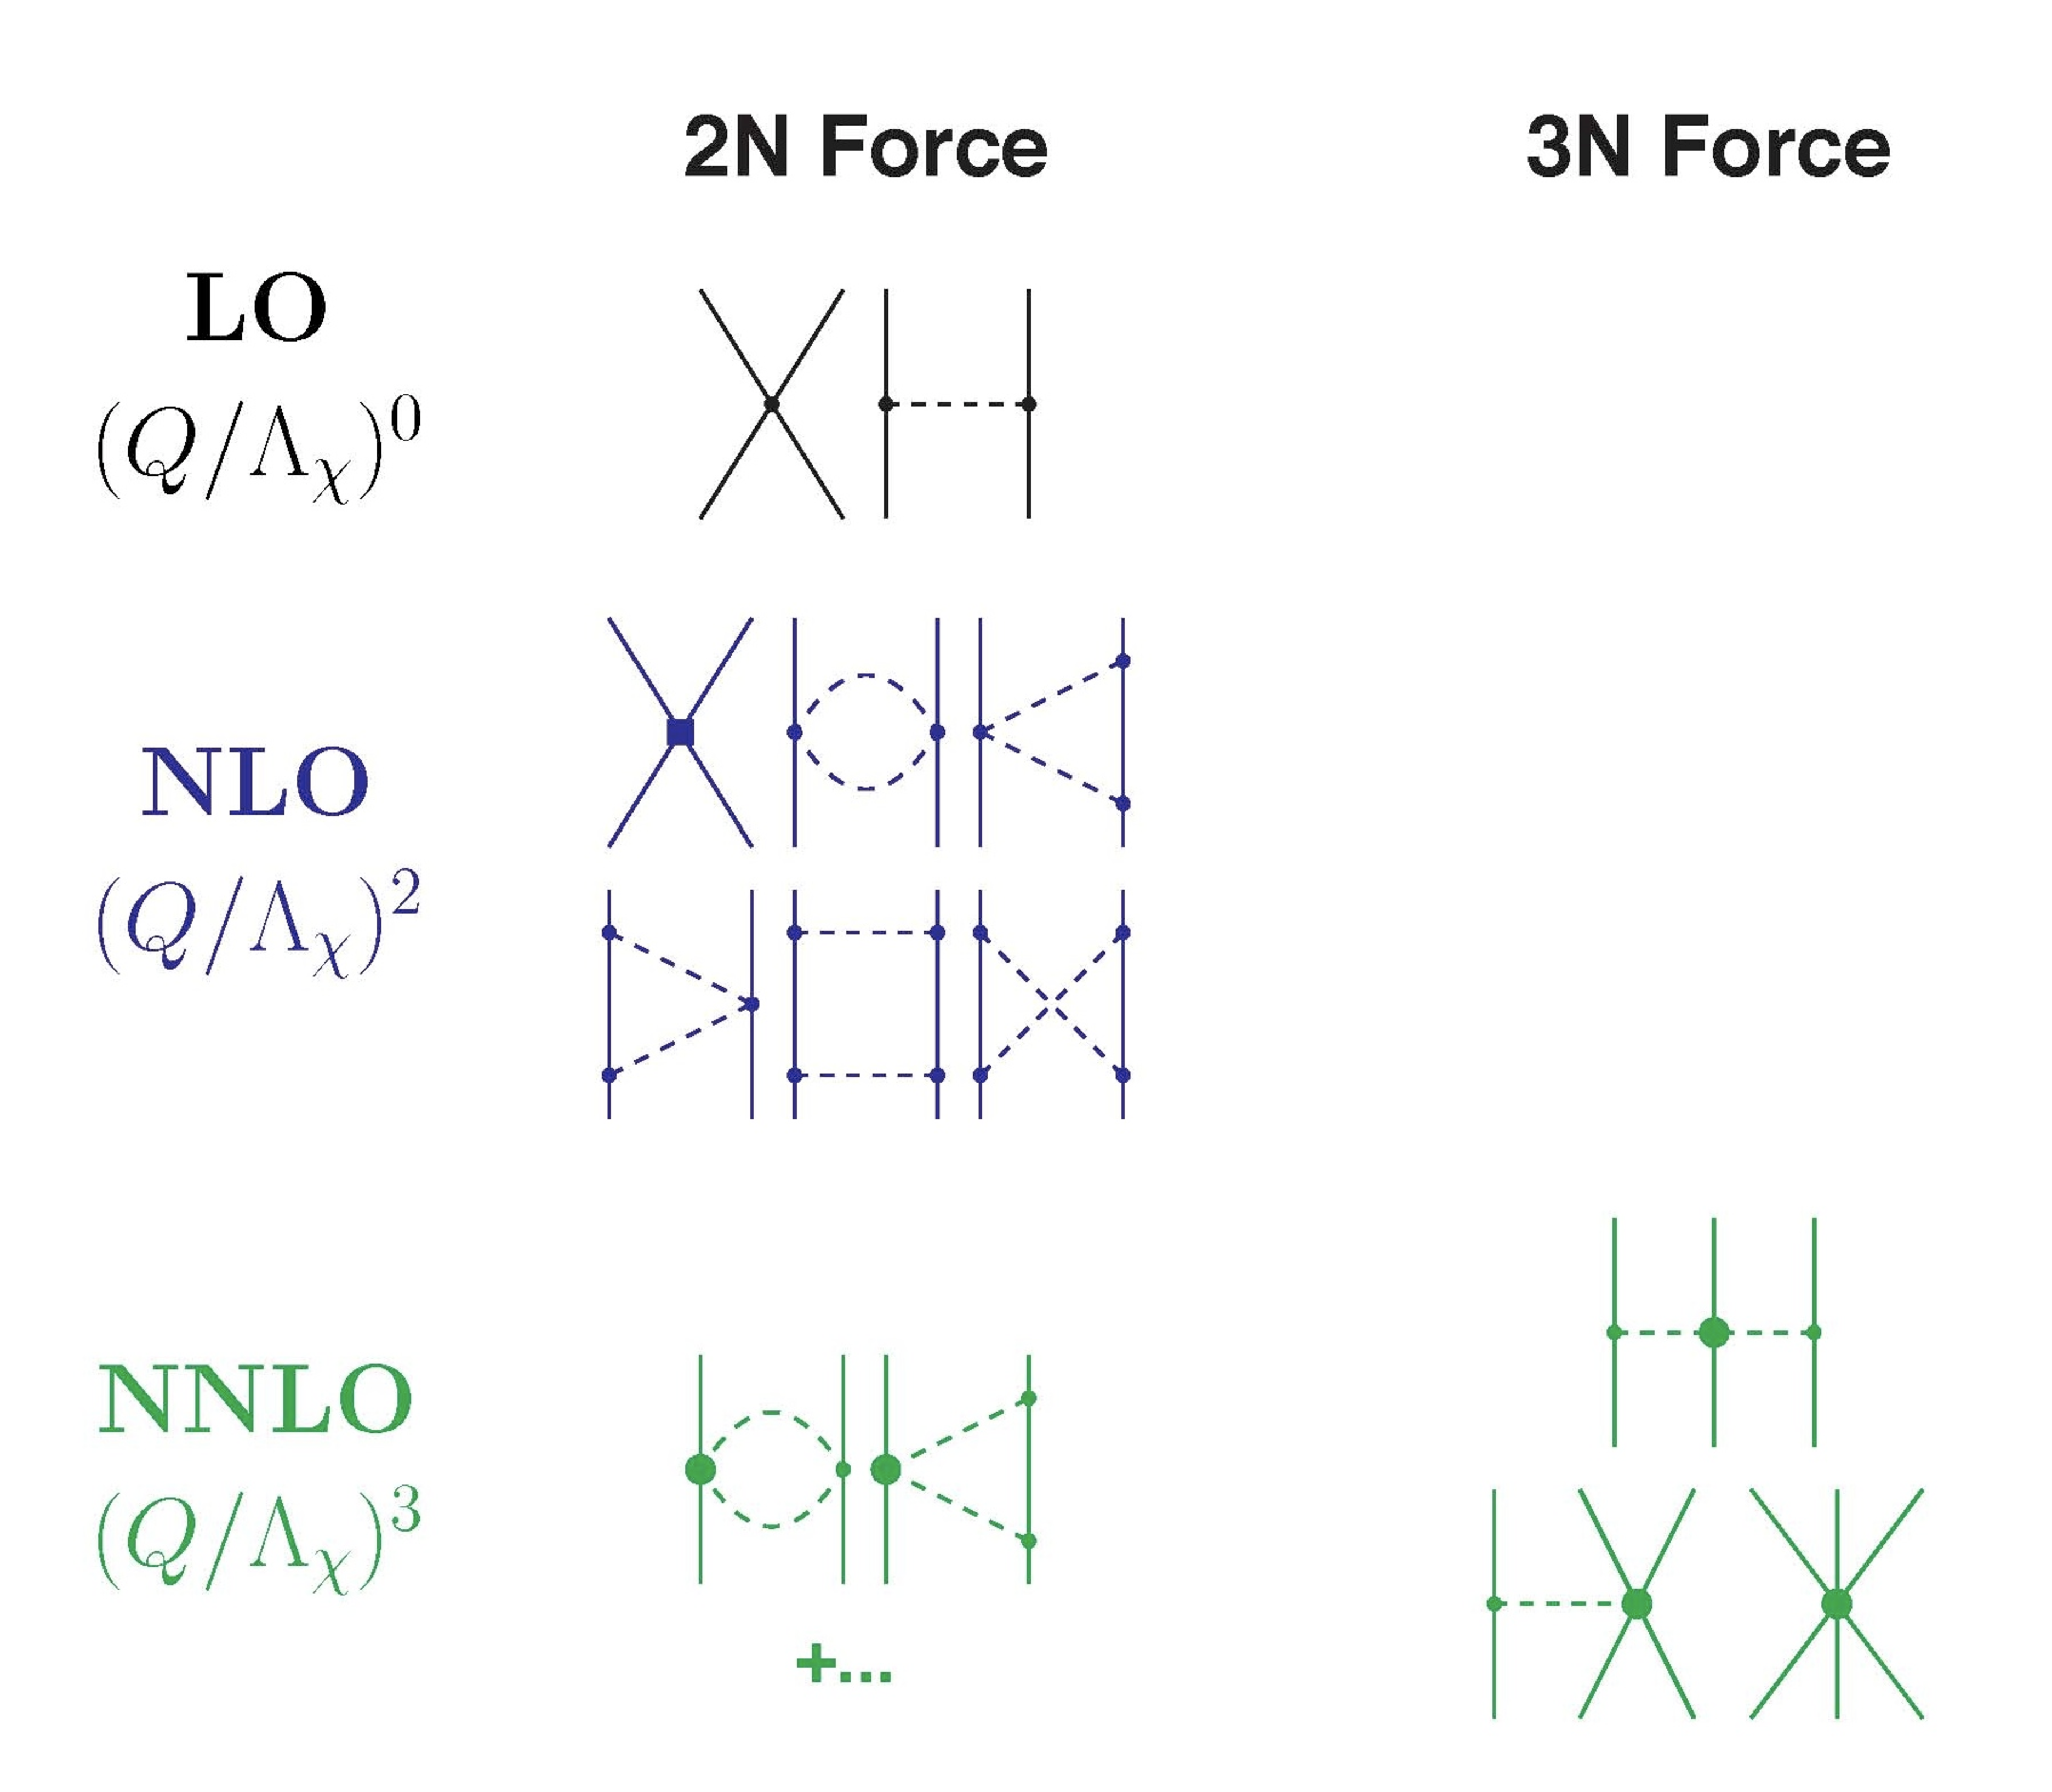
\includegraphics{Figs/diagNNLO.pdf}}
%\vspace*{-1.0cm}
\caption{Nuclear forces in ChPT up to NNLO. Solid lines
represent nucleons and dashed lines pions. 
Small dots, large solid dots, and solid squares
denote vertices of index $\Delta_i= \, $ 0, 1, and 2, respectively.}
\label{fig_diagNNLO}
\end{figure}
For an irreducible $NN$ diagram (``two-nucleon potential'', $A=2$, $C=1$),
Eq.~(\ref{eq_nu}) collapses to
\begin{equation} 
\nu =  2L + \sum_i \Delta_i \, .  
\label{eq_nunn} 
\end{equation}
Thus, in terms of naive dimensional analysis or ``Weinberg counting'' \cite{weinberg1990,weinberg1991},
the various orders of the irreducible graphs which define the chiral 
$NN$ potential 
are given by (cf.\ Fig.~\ref{fig_diagNNLO})
\begin{eqnarray}
V_{\rm LO} & = & 
V_{\rm ct}^{(0)} + 
V_{1\pi}^{(0)} 
\label{eq_VLO}
\\
V_{\rm NLO} & = & V_{\rm LO} +
V_{\rm ct}^{(2)} + 
V_{1\pi}^{(2)} +
V_{2\pi}^{(2)} 
\label{eq_VNLO}
\\
V_{\rm NNLO} & = & V_{\rm NLO} +
V_{1\pi}^{(3)} + 
V_{2\pi}^{(3)} 
\label{eq_VNNLO}
\end{eqnarray}
where 
the superscript denotes the order $\nu$ of the low-momentum expansion.
LO stands for leading order, NLO for next-to-leading
order and NNLO stands for next-to-next-to leading order.
Contact potentials carry the subscript ``ct'' and
pion-exchange potentials can be identified by an obvious subscript.

The charge-independent one-pion-exchange (1PE) potential reads
\begin{equation}
V_{1\pi} ({\vec p}~', \vec p) = - 
%\frac{1}{(2\pi)^3} \,
\frac{g_A^2}{4f_\pi^2}
\: 
{\vec \tau}_1 \cdot {\vec \tau}_2 
\:
\frac{
\vec \sigma_1 \cdot \vec q \,\, \vec \sigma_2 \cdot \vec q}
{q^2 + m_\pi^2} 
\,,
\label{eq:eq_1PEci}
\end{equation}
where ${\vec p}~'$ and $\vec p$ designate the final and initial
nucleon momenta in the center-of-mass system (CMS) and $\vec q \equiv
{\vec p}~' - \vec p$ is the momentum transfer; $\vec \sigma_{1,2}$ and
$\vec tau_{1,2}$ are the spin and isospin operators of nucleon 1 and
2; $g_A$, $f_\pi$, and $m_\pi$ denote axial-vector coupling constant,
the pion decay constant, and the pion mass, respectively. As in Ref.~\cite{carlsson2014}, we use
$f_\pi=92.4$ MeV and $g_A=1.29$ throughout this work.  
Since higher order corrections contribute only to mass
and coupling constant renormalizations and since, on shell, there are
no relativistic corrections, the on-shell 1PE has the form
of Eq.~(\ref{eq:eq_1PEci}) to all orders.

It is well known that, for high-precision $NN$ potentials,
charge dependence is important.
Therefore, we will 
take the charge dependence of the 1PE into account.
Defining a pion-mass dependent 1PE by
\[
V_{1\pi} (m_\pi) \equiv - \,
%\frac{1}{(2\pi)^3} \,
\frac{g_A^2}{4f_\pi^2} \,
\frac{
\vec \sigma_1 \cdot \vec q \,\, \vec \sigma_2 \cdot \vec q}
{q^2 + m_\pi^2} 
\,,
\]
the 1PE for proton-proton ($pp$) and neutron-neutron ($nn$)
scattering is
\[
V_{1\pi}^{(pp)} ({\vec p}~', \vec p) = 
V_{1\pi}^{(nn)} ({\vec p}~', \vec p) =
V_{1\pi} (m_{\pi^0}) \,,
\]
while for neutron-proton ($np$) scattering we have
\[
V_{1\pi}^{(np)} ({\vec p}~', \vec p) 
= -V_{1\pi} (m_{\pi^0}) + (-1)^{T+1}\, 2\, V_{1\pi} (m_{\pi^\pm})
\,,
\]
where $T$ denotes the isospin of the two-nucleon system.
We use $m_{\pi^0}=134.9766$ MeV and
 $m_{\pi^\pm}=139.5702$ MeV.
For the leading-order, next-to-leading order and NNLO, we refer the reader to Refs.~\cite{machleidt2011,carlsson2014}.
The final interaction at order NNLO is multiplied with the following factors \cite{machleidt2011},
\begin{equation}
\widehat{V}({\vec p}~',{\vec p})
\equiv 
\frac{1}{(2\pi)^3}
\sqrt{\frac{M_N}{E_{p'}}}\:  
{V}({\vec p}~',{\vec p})\:
 \sqrt{\frac{M_N}{E_{p}}}
\label{eq_minrel1}
\end{equation}
with $E_p=\sqrt{M_N^2+p^2}$ and
where the factor $1/(2\pi)^3$ is just added for convenience.
The potential $\widehat{V}$ satisfies the nonrelativistic
Lippmann-Schwinger (LS) equation,
\begin{equation}
 \widehat{T}({\vec p}~',{\vec p})= \widehat{V}({\vec p}~',{\vec p})+
\int d^3p''\:
\widehat{V}({\vec p}~',{\vec p}~'')\:
\frac{M_N}
{{ p}^{2}-{p''}^{2}+i\epsilon}\:
\widehat{T}({\vec p}~'',{\vec p}) \, .
\label{eq_LS}
\end{equation}
In $pp$ scattering, we use $M_N=M_p=938.2720$ MeV,
and in $nn$ scattering, $M_N=M_n=939.5653$ MeV.
Moreover, the on-shell momentum is simply
\begin{equation}
p^2  =  \frac12 M_N T_{\rm lab} \,,
\end{equation}
where $T_{\rm lab}$ denotes 
the kinetic energy of the incident nucleon 
in the laboratory system (``Lab.\ Energy'').
For $np$ scattering, we have
\begin{eqnarray}
M_N  &=&  \frac{2M_pM_n}{M_p+M_n} = 938.9182 \mbox{ MeV, and}
\\
p^2 & = & \frac{M_p^2 T_{\rm lab} (T_{\rm lab} + 2M_n)}
               {(M_p + M_n)^2 + 2T_{\rm lab} M_p}  
\,,
\end{eqnarray}
which is based upon relativistic kinematics.

Iteration of $\widehat V$ in the LS equation, Eq.~(\ref{eq_LS}),
requires cutting $\widehat V$ off for high momenta to avoid infinities.
This is consistent with the fact that ChPT
is a low-momentum expansion which
is valid only for momenta $Q \ll \Lambda_\chi \approx 1$ GeV.
Therefore, the potential $\widehat V$
is multiplied
with the regulator function $f(p',p)$,
\begin{equation}
{\widehat V}(\vec{ p}~',{\vec p})
\longmapsto
{\widehat V}(\vec{ p}~',{\vec p}) \, f(p',p) 
\end{equation}
with
\begin{equation}
f(p',p) = \exp[-(p'/\Lambda)^{2n}-(p/\Lambda)^{2n}] \,.
\label{eq:eq_f}
\end{equation}

One of the aims of this work is to test both the regulator dependence and the cutoff dependence at order NNLO, with and without 
three-body force. We have optimised nuclear forces at order NNLO for a series of cutoffs  $\Lambda$ MeV
and values of $n$ in Eq.~(\ref{eq:eq_f}). These are {\bf here we need to decide the amount of data we wish to study...}.

Up to NNLO in chiral perturbation theory there are, in addition to the
two-body interaction diagrams discussed above, also a few three-body
interaction diagrams, see Fig.~\ref{fig_diagNNLO}. In
chiral perturbation theory, the orders are generated systematically,
and at a given chiral order the number of Feynman diagrams is
finite. Consistency requires that a calculation includes all diagrams
which are present at the chosen order. In this work we employ 
chirally consistent many-body calculations including all NNLO nuclear
interactions.

There are in total five contact terms that determine the strength of the NNLO
three-nucleon force (3NF); $c_1,c_3,$ and $c_4$ are associated with
the three-body two-pion-exchange (2PE) diagram, $c_D$ and $c_E$
determine the strength of the one-pion-exchange plus contact (1PE)
diagram and the pure contact (CNT) diagram, respectively. Following
the notation of Ref.~\cite{epelbaum2002} the three-body diagrams are given
by
\begin{equation}
V^{\textnormal{2PE}}_{ijk} = \sum_{i \neq j \neq k} \frac{1}{2} \left( \frac{g_A}{f_{\pi}} \right)^2 \frac{(\vec{\sigma_i} \cdot \vec{q_i})(\vec{\sigma_j}\cdot \vec{q_j})}{(\vec{q_i}^2 + m_{\pi)}^2)(\vec{q_j}^2 + m_{\pi)}^2)} F_{ijk}^{\alpha \beta} \tau_i^{\alpha}\tau_{j}^{\beta} \,,
\end{equation}
where $q_{i}$ denotes the momentum transfer associated with nucleon $i$, and
\begin{align}
F_{ijk}^{\alpha \beta} ={}&  \delta^{\alpha \beta} \left[ -\frac{4c_1m_{\pi}^2}{f_{\pi}^2} + \frac{2c_3}{f_{\pi}^2}\vec{q_i}\cdot \vec{q_j}\right]\\
{}&+\sum_{\gamma}\frac{c_4}{f_{\pi}^2}\epsilon^{\alpha \beta \gamma} \tau_{k}^{\gamma} \vec{\sigma_k} \cdot [\vec{q_i} \times \vec{q_j}] \,.
\end{align}
For this diagram, no new parameters are introduced since the $c_1,c_3,c_4$ appear already in the 2PE two-nucleon interaction. The remaining two three-body terms are given by
\begin{equation}
V^{\textnormal{1PE}}_{ijk} = -\sum_{i \neq j \neq k} \frac{g_A}{8f_{\pi}^2} \frac{c_D}{f_{\pi}^2\Lambda_{\chi}} \frac{ (\vec{\sigma_j} \cdot \vec{q_j})}{(\vec{q_j}^2 + m_{\pi}^2)} (\tau_i \cdot \tau_j)(\vec{\sigma_i}\cdot \vec{\sigma_j})
\end{equation}
and
\begin{equation}
V^{\textnormal{CNT}}_{ijk} = \frac{1}{2}\sum_{i \neq j \neq k} \frac{c_E}{f_{\pi}^4 \Lambda_{\chi}} (\tau_i \cdot \tau_j) 
\end{equation}
with $\Lambda_{\chi}=700$ MeV. Following~\cite{navratil2007}, we use a regulator depending on the momentum-transfer $q$, 
\begin{equation}
f(q) = \exp[-q^4/\Lambda]
\end{equation}
and thus obtain a local three-body force. 




\subsubsection{Optimizing the nuclear interactions at NNLO using POUNDerS}

In Ref.~\cite{carlsson2014}, we made an extensive study of the optimization of nuclear forces up to next-to-next-to leading order 
{\bf Andreas, can you fill in briefly some details here?}


\subsubsection{Many-body perturbation theory and Coupled-Cluster theory}
{\bf shall we limit ourselves to HF only in the studies of the evolution of sp-energies?  This can be a paper by itself!}

\section{Results}\label{sec:results}


\begin{figure}%[hbtp]
     \begin{center}
        \subfigure[Results for the $0f_{7/2}$ single-particle state]{
            \label{fig:f72}
            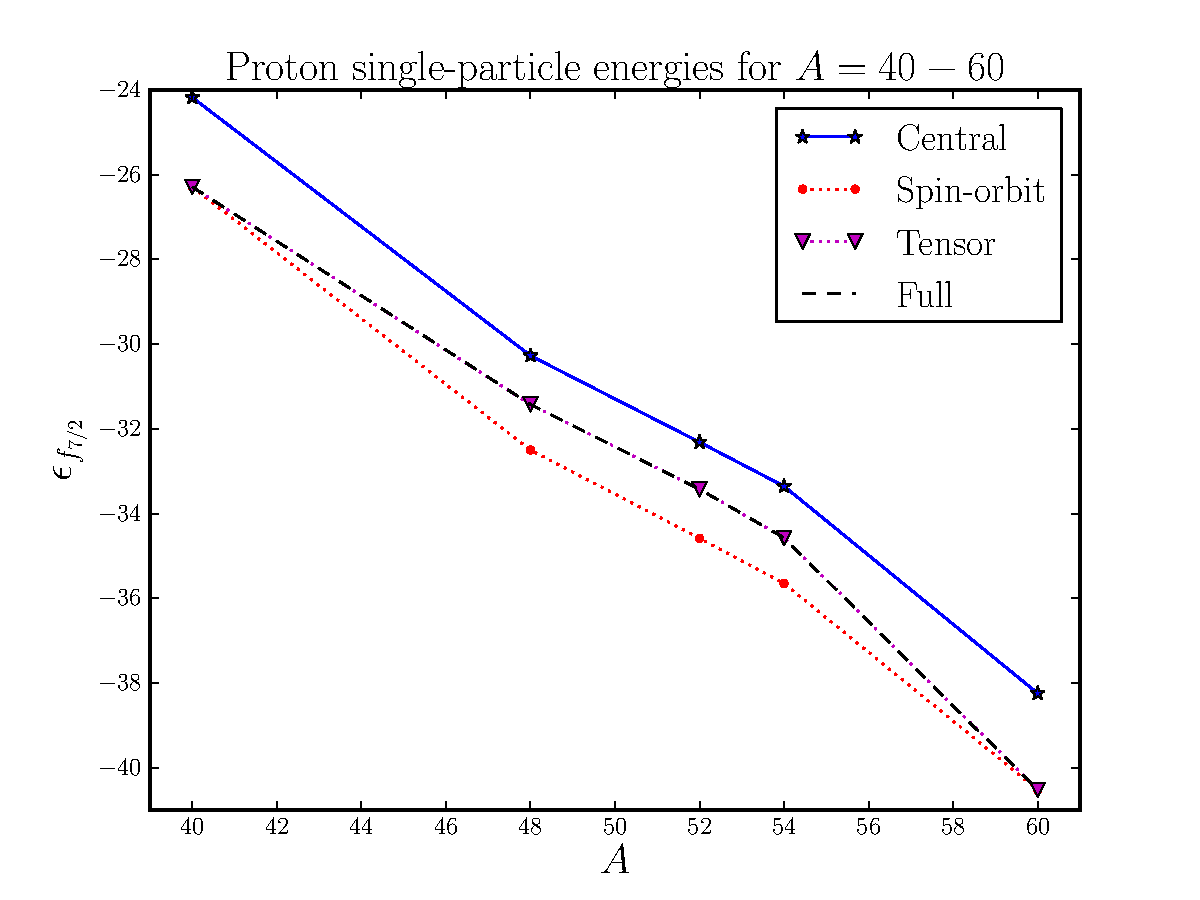
\includegraphics[width=0.38\textwidth]{Figs/protonf72.pdf}
        }
        \subfigure[Results for the $0f_{5/2}$ single-particle state ]{
           \label{fig:f52}
           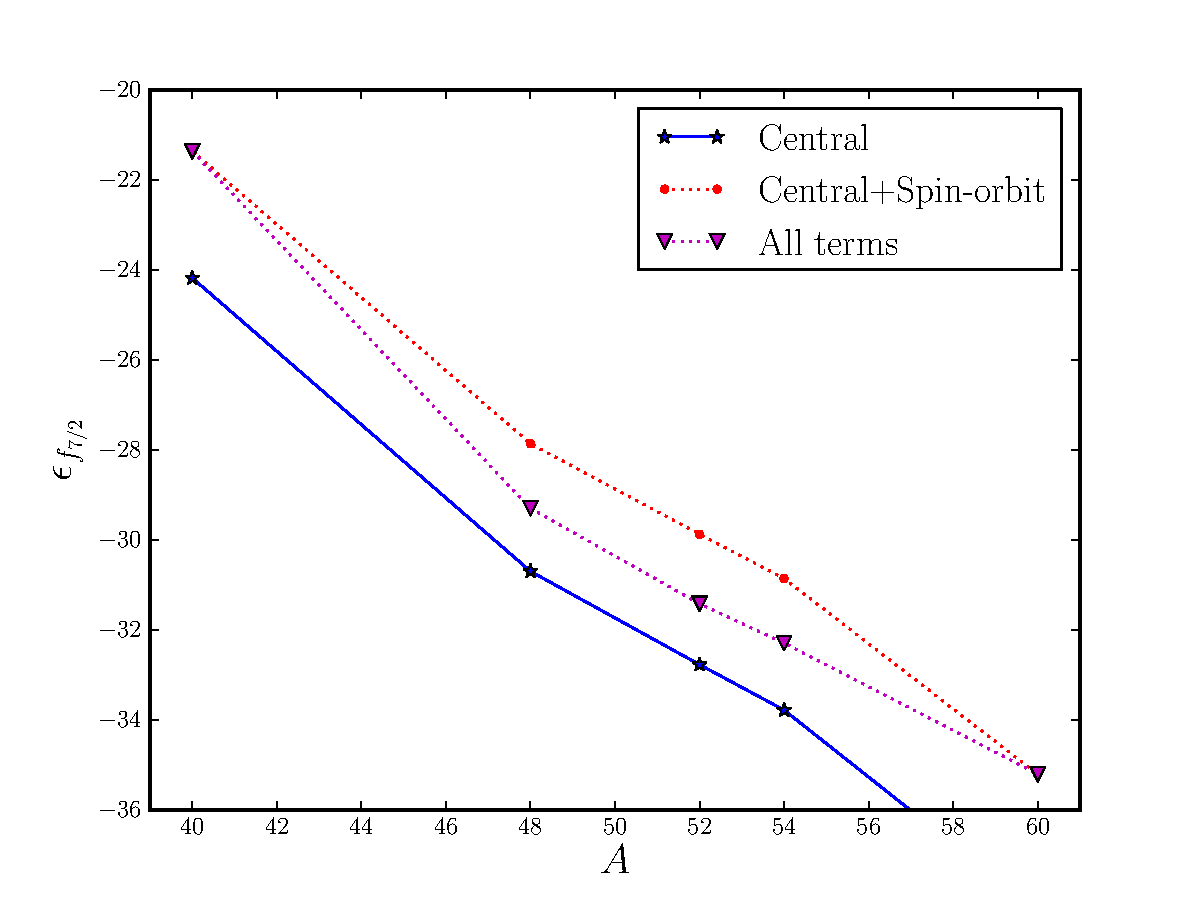
\includegraphics[width=0.38\textwidth]{Figs/protonf52.pdf}
        }\\ %  ------- End of the first row ----------------------%
        \subfigure[Results for the $1p_{3/2}$ single-particle state]{
            \label{fig:p32}
            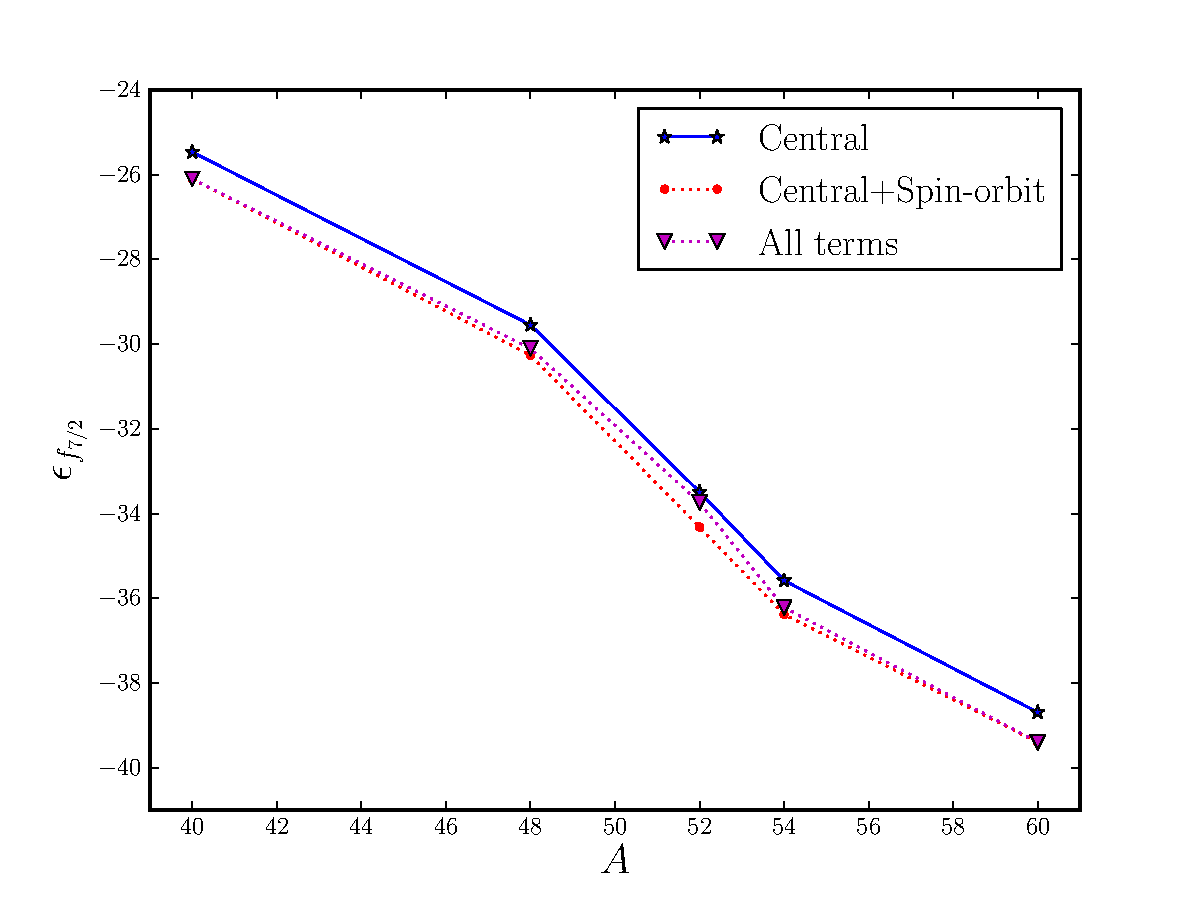
\includegraphics[width=0.38\textwidth]{Figs/protonp32.pdf}
        }
        \subfigure[Results for the $1p_{1/2}$ single-particle state]{
            \label{fig:p12}
            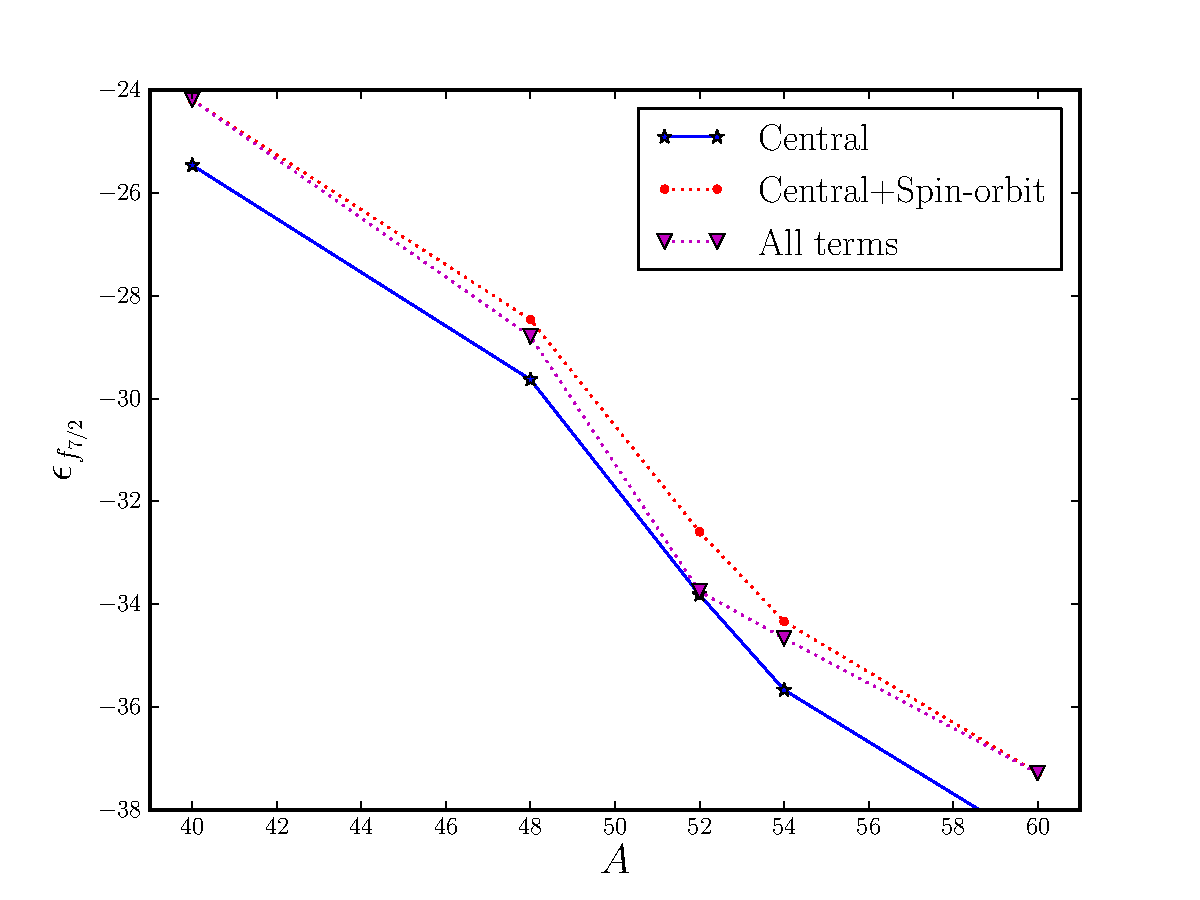
\includegraphics[width=0.38\textwidth]{Figs/protonp12.pdf}
        }
    \end{center}
\caption{Contributions from the central, spin-orbit and tensor components to  
the proton single-particle energies of $1p0f$ single-particle states. 
The closed-shell cores are $^{40}$Ca, $^{48}$Ca, $^{52}$Ca, 
$^{54}$Ca and $^{60}$Ca. The results have been obtained with a harmonic oscillator basis and an 
oscillator energy $\hbar\omega =10.5$ MeV using the N$^3$LO interaction model of Ref.~\cite{machleidt2011}.}
\label{fig:hoprotonCa}
\end{figure}


\section{Conclusions and perspectives}\label{sec:conclusions}




\begin{acknowledgments}
  This work was supported by the Office of Nuclear Physics,
  U.S.~Department of Energy (Oak Ridge National Laboratory). This research used computational resources of the
  National Center for Computational Sciences, the National Institute
  for Computational Sciences, the Notur project in Norway and the Research Council of Norway under project ISP-Fysikk/216699. 
\end{acknowledgments}


\bibliography{paper}
\bibliographystyle{apsrev}



\end{document}

 






